\subsubsection{Overview}

In this research, a new generation predictive system architecture has been developed. The main focus
of this paper is the creation of a thematic modeling system and analytical interface for the financial
subject area. A logical extension would be to build an interpretable and efficient predictive model based
on the thematic tone of financial publications (news articles, press releases, posts, transcripts, etc.).
Thus, the present work not only demonstrates the functioning principles of the basic module, but also
formulates a vision of how it can be extended with asset price prediction capabilities.

The proposed architecture relies on proven robust mixed prediction approaches --- a combination of convolutional
and recurrent neural networks (CNN-LSTM) \parencite{Hochreiter1997LSTM, CNN1998lecun, CNN_LSTM2020finance}. This solution
allows simultaneous consideration of global long-term trends (such as the overall market trend) and local short-term
patterns (such as head-and-shoulders, double bottoms, and other behavioral economics-driven structures).

It is important to keep in mind the variety of input data. Exchange metrics (Open, High, Low, Close, Volume, etc.)
and derived technical indicators (RSI, MACD, etc.) are usually used for forecasting. Our study adds textual data
as an Over The Counter (OTC) source. In the future, graph representations of links, images, audio and video
recordings can be attracted as additional modalities. Thus, at the current stage we work with three modalities,
each of which carries an independent semantic load and is able to explain price dynamics independently,
but their interaction can both amplify the useful signal and introduce noise.

There are three commonly accepted mechanisms for multimodal data fusion. The first, Early Fusion, involves feeding
all features (stock quotes, technical indicators, and textual embeddings) at once into a single CNN-LSTM model
\parencite{Karpathy_2014_CVPR, dutt2022shared}. The advantage of the method is the ease of implementation and the ability
to immediately learn cross-modal dependencies. However, in practice Early Fusion is prone to “choking” in the noise
of one of the modalities and loses flexibility when dynamically estimating the contribution of each modality
\parencite{dutt2022shared}.

The second method, Late Fusion, combines the predictions of individual channels (each modality is processed by its
CNN-LSTM branch) only at the final stage \parencite{Karpathy_2014_CVPR, ortega2019multimodal}. This approach is characterized
by modularity (easy replacement or additional training of a single channel), but it excludes extraction of low-level
cross-modal patterns and requires training all branches separately, which entails a multiple increase in computational
resources \parencite{joze2020mmtm}.

The third, compromise mechanism, Slow Fusion, provides staged, “slow” merging of links at different layers of the network
\parencite{feichtenhofer2016convolutional, dutt2022shared}. Slow Fusion approaches Early Fusion for early merging, and Late Fusion
for late merging. The key advantages of the method are: the balance between the autonomous processing of each modality
and the possibility of taking into account their interaction, preserving the “purity” of low-level features and
the flexibility of setting the number and depth of integration stages \parencite{Karpathy_2014_CVPR}. The main disadvantages
are the difficulty of choosing the optimal fusion level and increased computational costs due to parallel branches
at early layers, but nevertheless, less than in Late Fusion.

In this study, the architecture was based on CNN-LSTM using Slow Fusion. The main engineering challenge was to harmonize
the spatio-temporal shapes of features of different modalities. To address this challenge, the architecture introduced
a Feature Caching Mechanism block that synchronizes the tone vectors of the textual modality with the stock time series.

Additionally, the textual branch is preprocessed: based on the developed thematic modeling system, the thematic tones
of publications are computed. This allows obtaining specialized scores for each topic, which gives an advantage over
the use of a single common tone.

\begin{figure}[H]
    \centering
    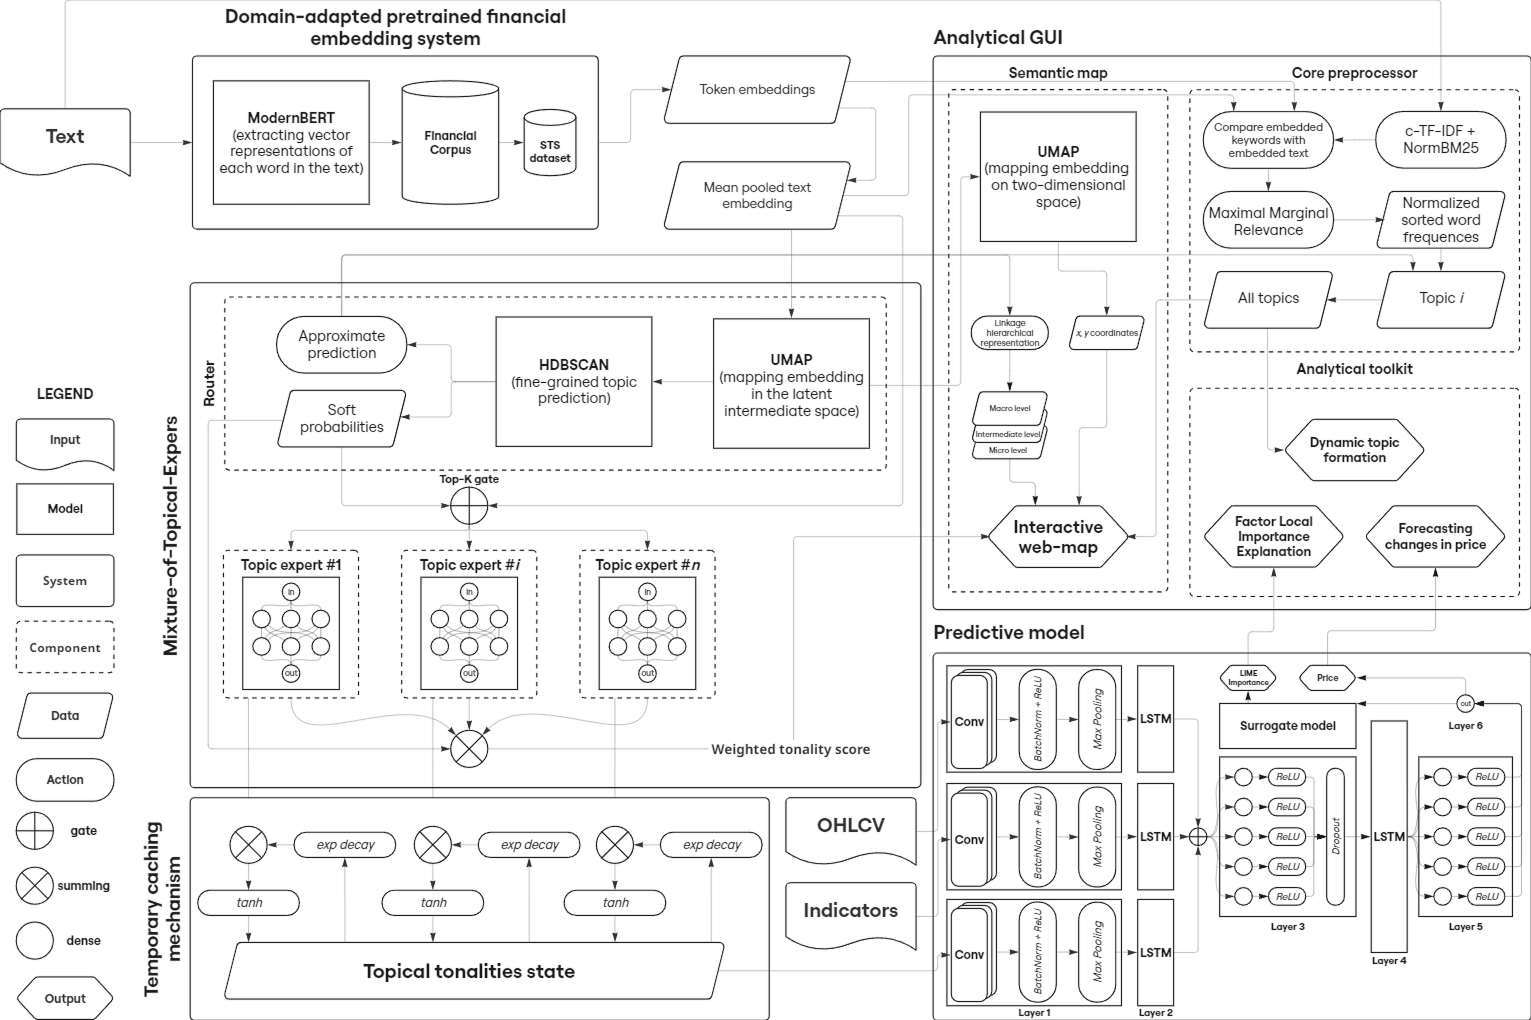
\includegraphics[width=1\linewidth]{img/architecture_overview.png}
    \caption{Overview of Financial Aspect-Based hybrid Semantic System (FinABYSS) architecture.}
    \label{fig:architecture_overview}
\end{figure}

The designed system consists of five main modules (Figure \ref{fig:architecture_overview}):

\begin{itemize}
    \item A financial language model (domain-adapted, fine-tuned for the STS task) that produces vector representations
    of the whole text and for each token.
    \item A Mixture-of-Topical-Experts that shapes the tone of the publication for each topic.
    \item A Temporal Caching Mechanism that aligns topic vectors to timestamps of stock data.
    \item A kernel predictive model with CNN-LSTM and Slow Fusion that processes all modalities and predicts asset price.
    \item An analytical GUI that aggregates intermediate results for further financial analysis.
\end{itemize}

Thus, the developed architecture is a powerful and adaptable tool for predicting the value of financial assets
based on a comprehensive evaluation of the thematic sentiment of publications.

\subsubsection{Embedding System}
Proceeding to the consideration of individual blocks of the developed architecture, we should start with the stage
of data preprocessing. The most resource-intensive and complex of them is the preparation of OTC text sources.

Immediately after entering the system, the text undergoes primary processing with the help of a domain-adapted
financial embedding model configured for the task of semantic text comparison (STS). This model extracts vector
representations for each token, thus preserving subtle contextual relationships within sentences. As new versions
of embedding models become available, it is important to regularly update the underlying model and re-adapt it
to the specifics of the financial domain.

The simplest path of domain adaptation involves an additional training stage on a Masked Language Modeling (MLM)
task. The corpus of financial publications generated in this study or its extended version, as well as other relevant
text corpora, can be used as a corpus for this purpose. For fine-tuning for the STS task, small labeled datasets
are sometimes used, but to save resources it is possible to do without them, using contrastive learning methods
on random subsamples of the main corpus \parencite{gao2021simcse}.

Once the token embeddings are extracted, they are aggregated: usually averaging is applied, which gives a vector
representation of the whole document. Then the document and its embeddings (both tokens and the averaged vector)
are passed to the analysis module for visualization and interpretation of the results. In parallel, the document
vector is sent to the “Mixture-of-Topical-Experts” block, where the topic tones of the publication are generated
based on it.

As a concrete implementation, this study uses the 'gte-modernbert-base' model built on the ModernBERT architecture.
Although it did not undergo domain adaptation initially, it shows high performance: the clustering of embeddings
yielded a DBCV index of 0.485, and visual and contextual analysis showed a clear separation of thematic groups.

Thus, the proposed preprocessing step provides:

\begin{itemize}
    \item Preserving deep semantic relations at the token and whole document level.
    \item Flexibility and reproducibility of the model adaptation process to the financial corpus.
    \item Integration of the results into the neighboring blocks of the architecture --- a Mixture-of-Topical-Experts
    and analytical GUI system.
\end{itemize}

\subsubsection{Mixture-of-Topical-Experts}

This block utilizes a state-of-the-art Mixture-of-Experts (MoE) architecture that has been successfully
applied in large language models (e.g., Mixtral 8×7B, DeepSeek R1) and in Google research (Switch Transformer)
\parencite{fedus2022switch}. The main components, a learning router and multiple experts, allow only a small fraction
of parameters to be dynamically activated at inference, ensuring high throughput and efficiency
\parencite{shazeer2017outrageously}. Especially for the analysis of financial texts, the experts are thematically
specialized, which increases interpretability and accuracy in assessing the tone of publications.

MoE architecture is based on the principle of conditional computation: only a part of subnets (“experts”) is active
for each input example, which reduces computational costs at a huge total number of parameters
\parencite{shazeer2017outrageously}.

\begin{itemize}
    \item The router (gating network) receives the embedding of a document as input and computes a distribution
    of “weights” for all experts, then selects either the top-K experts or those whose weight exceeds a threshold
    \parencite{fedus2022switch}.
    \item Experts are shallow feed-forward networks, each specializing in a different topic (in the context
    of the paper, one of the financial topics) \parencite{shazeer2017outrageously}.
\end{itemize}

When processing each embedding, only a small fraction of experts are activated --- usually by Top $K$ (selecting $K$
of the most relevant experts) or by a threshold value (weighting the expert above a given threshold) --- making MoE
extremely computationally parsimonious with a colossal total number of parameters \parencite{fedus2022switch}.
The values of $K$ and $\theta$ act as hyperparameters and are customized on validation data.

For analyzing financial texts, the MoE model is a logical choice, since publications often contain a mixture
of related topics (macroeconomics, corporate reports, geopolitics, etc.), and it is necessary to evaluate the tone
from different angles. Experts make it possible to form specialized assessments for each topic simultaneously,
preserving the “purity” of low-level processing and ensuring the interpretability of the results \parencite{jacobs1991adaptive}.
Nevertheless, it is also worth noting the high complexity of selecting $K$ or $\theta$ hyperparameters
\parencite{jacobs1991adaptive}.

Instead of training experts on subjectively labeled data, their parameters are optimized by back propagation of the error
coming from the asset price prediction unit. This ensures that each expert is trained directly on the impact of publications
on asset prices rather than on external annotations \parencite{shazeer2017outrageously}. Once topic tones are obtained,
they are aggregated by weighted summation considering topic probabilities, normalized, and sent to the analytics system
for visualization, and to the feature caching engine for synchronization with exchange data.

Thus, the MoE-based Mixture-of-Topical-Experts block provides a combination of scalability, efficiency, and interpretability
in analyzing financial texts. The dynamic activation of a small number of experts allows processing huge models without
a proportional increase in computation, and training the experts through the signal from the price prediction model makes
the estimation of tones objective and close to the economic reality. Thus, the proposed architecture opens up new opportunities
for accurate prediction and in-depth analysis of the impact of textual publications on the value of financial assets.

\subsubsection{Feature Caching Mechanism}
The Feature Caching Mechanism is the central component of the architecture that ensures synchronization
between exchange data (regularly arriving time series) and over-the-counter textual “ticks” scattered
in time. When a new assessment of the tone of a publication on topic $i$ arrives from the Mixture-of-Topical-Experts
block, it is instantly added to the matrix of accumulative exponentially smoothed values by Equation \ref{eq:exp_decay}:

\begin{equation}\label{eq:exp_decay}
    x_{i,t}=x_{i, t-1} + x_{i, 0} \cdot e^{-\lambda \cdot t},
\end{equation}

where $x_{i, 0}$ is the initial tone on topic $i$, $x_{i,t-1}$ is the previous smoothed value, and $\lambda$
is the hyperparameter of the rate of exponential “fading” of the signal. This approach reflects the lagged
and time-smoothed response of market participants to publications.

This approach takes into account that market participants' reaction to information events is delayed
and distributed in time: the first “wave” of perception fades quickly, followed by smoother and longer
effects, which in finance is traditionally modeled by exponential decline.

Since the original tones are normalized in the range $[-1,1]$, the cumulative summation by the
Equation \ref{eq:exp_decay} can go beyond these bounds. To keep the scaling within acceptable
intervals and to make the accumulation smooth, we propose to re-normalize the results using
a hyperbolic tangent (Equation \ref{eq:tanh1}):

\begin{equation}\label{eq:tanh1}
    tone_{i, t} = \tanh(tone_{i, t-1} + x_{i,t}) =
    \cfrac{
        \tanh{(tone_{i, t-1})} + \tanh{(x_{i,t})}
    }{
        1 + \tanh{(tone_{i, t-1})} \cdot \tanh{(x_{i,t})}
    }.
\end{equation}

which is equivalent to Equation \ref{eq:tanh2}:

\begin{equation}\label{eq:tanh2}
    tone_{i, t} =
    \cfrac{
        (1-e^{-2 \cdot tone_{i, t}})+(1-e^{-2x_{i,t}} - (1-e^{-2 \cdot tone_{i, t}}) \cdot(1-e^{-2x_{i,t}})
    }{
        (1+e^{-2 \cdot tone_{i, t}})+(1+e^{-2x_{i,t}} - (1+e^{-2 \cdot tone_{i, t}}) \cdot(1+e^{-2x_{i,t}})
    },
\end{equation}

where $tone_{i, t}$ is the current normalized exponentially smoothed tone on topic $i$ at time $t$.

As a result of continuous operation of the Feature Caching Mechanism, a matrix of accumulative topic tonalities
is formed and updated at each arrival of a textual “tick”. While stock exchange data (Open, High, Low, Close,
Volume and indicators) are absent, this time series accumulates “market sentiment” signals. As soon as a new
time series of stock exchange measurements comes into the system (taking into account the network delay $\delta$),
the accumulated and normalized tones are concatenated with price and indicator data and passed to the Predictive
Model for joint processing.

The dynamic process of the mechanism is illustrated in the Image \ref{fig:feature_caching_mechanism}. At the input
moment, the cache is initialized with zero values, then it is updated with the first formula at each arrival
of textual evaluation, after which it is normalized with a hyperbolic tangent. When a trigger is reached --- moment
$t$ or stock data arrives at moment $t+\delta$ --- the merged time series is passed on.

\begin{figure}[H]
    \centering
    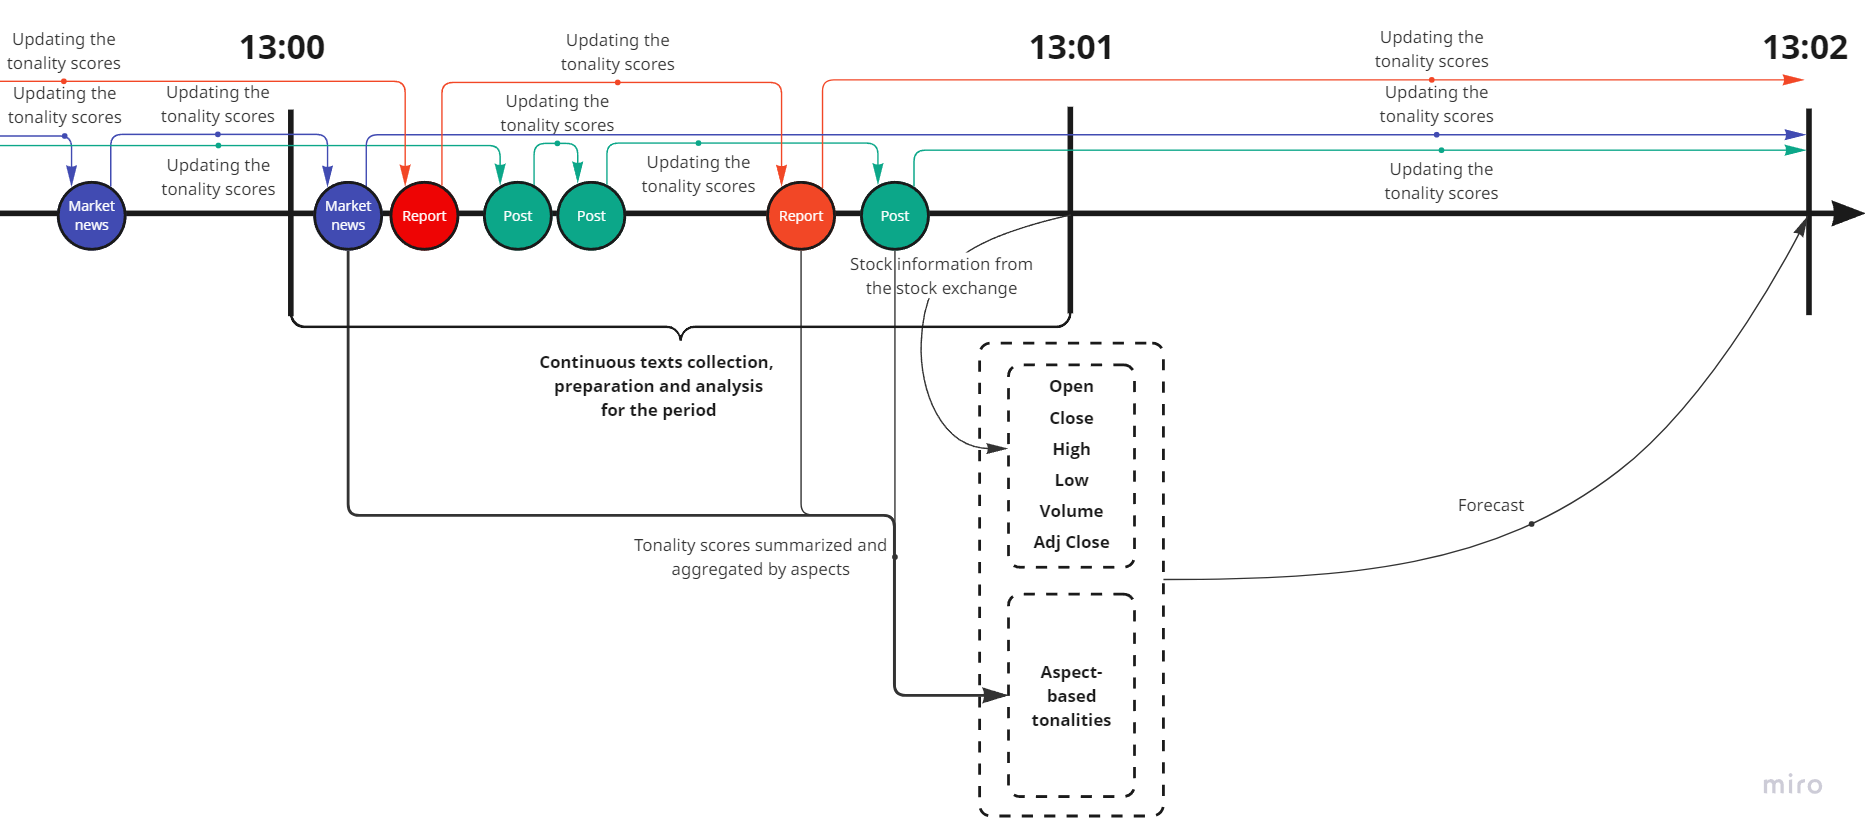
\includegraphics[width=1\linewidth]{img/feature_caching_mechanism.png}
    \caption{Dynamic representation of OTC data synchronization using Feature Caching Mechanism.}
    \label{fig:feature_caching_mechanism}
\end{figure}

Thus, the Feature Caching Mechanism performs the following functions: converts irregular textual events
into a continuous multidimensional time series, applies tone smoothing and scaling adequate to financial
realities, and guarantees synchronization with stock exchange data. This ensures consistency and stability
of input features in the Predictive Model and contributes to the accuracy of financial asset value forecasting.

\subsubsection{Predictive Model}
In the proposed hybrid architecture, we aim to combine the advantages of convolutional layers for local feature
extraction and recurrent modules for modeling long-range dependencies, while providing adaptive fusion of quantitative
and qualitative signals. The input is a multivariate time series of length $T$, in which each time step t corresponds
to a vector $x_t = [x_t^{\rm price}, x_t^{\rm ind}, x_t^{\rm sent}]$, where $x_t^{\rm price}\in\mathbb{R}^{C_p}$ contains
OHLCV, $x_t^{\rm ind}\in\mathbb{R}^{C_i}$, and $x_t^{\rm sent}\in\mathbb{R}^{C_s}$ is the set of sliding and smoothed
values of news tones.

The data is first split into three branches: Price, Indicator, and Sentiment. Each branch undergoes two basic levels
of processing. At the first level, in each branch, the sequence $\{x_t^{(\cdot)}\}_{t=1}^T$ is passed through
a 1D convolution with small kernels and pooling operations (Equation \ref{eq:relu_pooling})

\begin{equation}\label{eq:relu_pooling}
    y^{(\ell+1)}_{t} = \mathrm{ReLU}\bigl(W^{(\ell)} * y^{(\ell)}_{t} + b^{(\ell)}\bigr), \\
    y^{(\ell+\tfrac12)}_{t} = \max\bigl(y^{(\ell+1)}{t},\,y^{(\ell+1)}_{t+1}\bigr).
\end{equation}

where the symbol $*$ denotes time convolution, the activation function $\mathrm{ReLU}$ is defined as follows
(Equation \ref{eq:relu}):

\begin{equation}\label{eq:relu}
    \mathrm{ReLU}(x)=\max(0, x).
\end{equation}

The max pooling operation then halves the time dimensionality. This sequence allows the initial layers to identify
local patterns within each flow, be it short price swings, indicator pulses, or sentiment fluctuations.

Next, the output of the pooling in each branch is trained by a recurrent LSTM, which models the accumulation
and forgetting of information taking into account long time dependencies. Let $h_t$ and $c_t$ be the hidden state
and memory cell of the LSTM; their evolution is given by the standard input-, forget-, and output-gate equations.
This ensures that each branch learns independently to determine which local features are significant for prediction
at more distant time horizons.

After each branch has produced its hidden state $h_t^{\mathrm{price}}$, $h_t^{\mathrm{ind}}$, $h_t^{\mathrm{sent}}$
at each time step, an adaptive merging step takes place. For this purpose, the vector concatenation $u_t$ is passed
through the gate layer (Equation \ref{eq:gate})

\begin{equation}\label{eq:gate}
    g_t = \sigma\bigl(W_g\,u_t + b_g\bigr).
\end{equation}

where $\sigma$ is a sigmoid and $g_t\in(0,1)^{\dim u}$ specifies the element-by-element coefficients controlling
the relative contribution of each flux. The combined representation itself is computed as

\begin{equation}
    m_t = g_t\odot u_t + (1-g_t)\odot\mu(u_t).
\end{equation}

where $\mu(u_t)$ can be an averaging or other aggregator of the components of the vector $u_t$. This mechanism
allows the model to dynamically switch between emphasizing price patterns, indicator signals, or sentiment
depending on the context of a particular time period.

The merged sequence $\{m_t\}_{t=1}^{T/2}$ is then fed back into the recurrent module merge-LSTM, which, like
the previous ones, accumulates information about the joint development of the three modalities at a higher
level of abstraction. Its output is the last hidden state $h_{T/2}^{\mathrm{merge}}$, which contains
a concise summary of the whole story. To add nonlinearity and an extra dimension of expressiveness, this
state can be passed through a full-link layer with the $\mathrm{ReLU}$ function, and then through a Dropout
layer to regularize and mitigate overtraining.

Finally, the final layer without activation translates the resulting vector into a univariate prediction
$\hat y$, which is interpreted as a new price (in regression mode).

Also, it is worth noting that, for purposes of local interpretability of the tone estimates, an important
role in the architecture is played by the presence of a separate surrogate model that, based on a sampling
of a number of tones obtained from the FCM, with additional undulations, estimates the contribution
of each topical tone to the final asset value prediction.

Thus, the proposed hybrid architecture combines local pattern detection (1D convolutions), the ability
of LSTM to model long-term dependencies, and an adaptive fusion mechanism that allows dynamically adjusting
the contribution of price, indicator, and sentiment signals. This provides high forecast accuracy with moderate
computational complexity and transparency of the model with respect to the attributes used, while remaining
lighter and more transparent than its transform-based counterparts.

\subsubsection{Analytical Graphical User Interface}
\label{sec:gui}
To conclude the description of the FinABYSS architecture, it is necessary to dwell on the key user
component --- the Analytical Graphical User Interface (GUI). This module accumulates the results
of all previous stages: from pre-processing of OTC texts and their thematic interpretation in
the Mixture-of-Topical-Experts block to concatenation with price and indicator series in the predictive
model. The GUI inputs intermediate and final data, and its task is to bring them into a visual, interactive
and analytically relevant form. The GUI consists of three interrelated components that implement data
post-processing, provide deep analysis tools, and visualize semantic relationships between documents.

The first component, the Core Postprocessor, is responsible for transforming the “raw” outputs
of the previous blocks into ordered and compact representations. In the initialization phase, it computes
the relative frequencies of terms using a BM25-modification of TF-IDF and additional normalization, which
removes noise and frequently occurring but semantically insignificant tokens (e.g., names of aggregators
like Zacks). Next, after obtaining embeddings of tokens and the whole document from the domain-adapted
language model, $n$-grams are ranked by frequency, taking into account the cosine similarity between
the token vectors and the document vector. To ensure a balance between relevance and subsystem
diversification, the Maximal Marginal Relevance (MMR) algorithm is applied: when partitioning into bigrams,
MMR eliminates duplicate or redundantly close in meaning fragments, leaving the most informative ones. For
example, from raw bigrams “ai” and “ai stocks”, depending on the relative frequency and semantic proximity,
either “ai” and “stocks”, or only “ai stocks”, or only “ai” can be retained, which increases the homogeneity
of the final dictionary and reduces redundancy.

After MMR is applied, the dictionary is sorted by the resulting frequencies, and the postprocessor receives
from the Mixture-of-Topical-Experts block the label of the cluster to which the current document belongs.
Based on this cluster membership, incremental updating of c-TF-IDF statistics is performed: the accumulated
word frequencies within each cluster are adjusted to reflect new publication, which provides adaptability
and accounts for the evolution of thematic trends over time and is used for dynamic thematic modeling. Two
data streams are fed in parallel from the postprocessor: the enriched frequency features and other extracted
text metadata are sent to the Analytic Toolkit, and the cleaned and clusterred text with embeddings is sent
to the Semantic Map.

The second component --- Analytical Toolkit --- is a set of visual and interactive elements that allow
the user to explore in-depth the dynamics of thematic trends and their impact on asset prices. Through
the dashboards it is possible to receive:

\begin{itemize}
    \item historical tone charts for each topic, combined with price series and technical indicators;
    \item dynamic correlation matrices between news topics sentiments and price movements;
    \item summary reports on the impact of macro, meso and micro topics on volatility and trend movements;
    \item aggregated market sentiment indicators (weighted total tone across all topics) with trend lines.
\end{itemize}

The toolkit is designed with future expansion in mind: when adding new modalities (images, graph data, audio
or video streams), modality-specific widgets can be easily integrated — for example, interactive clouds of key
entities, graphs of relationships, or heat maps of sentiment in voice and video formats.

The third component, Semantic Map, implements two-dimensional visualization of document embeddings. Based
on a pre-trained dimensionality reduction model, each document representation from the latent space where
clustering was performed is mapped in $(x,y)$ coordinates. In parallel, an approximate topic predictor
from the Mixture-of-Topical-Experts block is used: for each document, a hierarchically organized triple
of topic labels is defined — on macro-, meso- and micro-versions. The color, size, and shape of the markers
on the map encode cluster membership, sentiment strength, and text volume. This allows to analyze not only
the spatial neighborhood of publications, but also their topical multilevel structure, quickly identify
peripheral and central documents, and track the evolution of topical communities.

Together, the GUI creates a single interactive panorama in which the results of the deepest computational
building blocks — from the Feature Caching Mechanism and Mixture-of-Topical-Experts to the hybrid CNN-LSTM
predictive model — are transformed into an intuitive and analytically rich tool. The user is able not only
to view price forecasts, but also to explore in detail the cause-and-effect relationships between media
signals and market movements.

The FinABYSS analytical GUI provides end-to-end visualization and interpretation of system output
by integrating frequency, topic, and embedding attributes into three interconnected subsystems. The kernel
postprocessor transforms raw textual and numerical data into compact and representative attributes,
the analytical toolkit offers flexible tools for in-depth exploration of the impact of topics on asset value,
and the semantic map provides a visualization of multidimensional embeddings based on hierarchical topics.
With this combination of technological power and interoperability, the GUI is the final but no less important
link in the forecasting pipeline, providing transparency, adaptability and visibility for financial experts.